%\documentclass[a4paper]{article}
\usepackage[utf8]{inputenc}
\usepackage[spanish, es-tabla, es-noshorthands]{babel}
\usepackage[table,xcdraw]{xcolor}
\usepackage[a4paper, footnotesep=1.25cm, headheight=1.25cm, top=2.54cm, left=2.54cm, bottom=2.54cm, right=2.54cm]{geometry}
%\geometry{showframe}

%\usepackage{wrapfig}			%Wrap figure in text
\usepackage[export]{adjustbox}	%Move images
\usepackage{changepage}			%Move tables

\usepackage{tikz}
\usepackage{amsmath}
\usepackage{amsfonts}
\usepackage{amssymb}
\usepackage{float}
\usepackage{graphicx}
\usepackage{caption}
\usepackage{subcaption}
\usepackage{multicol}
\usepackage{multirow}
\usepackage{wrapfig}
\setlength{\doublerulesep}{\arrayrulewidth}
\usepackage{booktabs}
\usepackage[numbib, nottoc, notlot, notlof]{tocbibind}

\usepackage{hyperref}
\hypersetup{
    colorlinks=true,
    linkcolor=blue,
    filecolor=magenta,      
    urlcolor=blue,
    citecolor=blue,    
}

%Change Font Size

% #1 = size, #2 = text
\newcommand{\setparagraphsize}[2]{{\fontsize{#1}{6}\selectfont#2 \par}}		%Cambia el size de todo el parrafo
\newcommand{\setlinesize}[2]{{\fontsize{#1}{6}\selectfont#2}}				%Cambia el font de una oración

\newcommand{\note}[1]{
	\begin{center}
		\huge{ \textcolor{red}{#1} }
	\end{center}
}

%FONTS (IMPORTANTE): Compilar en XeLaTex o LuaLaTeX
\usepackage{anyfontsize}	%Font size
\usepackage{fontspec}		%Font type

\usepackage{etoolbox}
\usepackage{todonotes}

\newcommand{\observacion}[2]{  \ifnumequal{1}{#1}{ { \todo[inline,backgroundcolor=red!25,bordercolor=red!100]{\textbf{Observación: #2}} } }{  }  }

\setcounter{topnumber}{2}
\setcounter{bottomnumber}{2}
\setcounter{totalnumber}{4}
\renewcommand{\topfraction}{0.85}
\renewcommand{\bottomfraction}{0.85}
\renewcommand{\textfraction}{0.15}
\renewcommand{\floatpagefraction}{0.8}
\renewcommand{\textfraction}{0.1}
\setlength{\floatsep}{5pt plus 2pt minus 2pt}
\setlength{\textfloatsep}{5pt plus 2pt minus 2pt}
\setlength{\intextsep}{5pt plus 2pt minus 2pt}

\newcommand{\quotes}[1]{``#1''}
\usepackage{array}
\newcolumntype{C}[1]{>{\centering\let\newline\\\arraybackslash\hspace{0pt}}m{#1}}
\usepackage[american]{circuitikz}
\usetikzlibrary{calc}
\usepackage{fancyhdr}
\usepackage{units} 

\graphicspath{{../Control de posición no lineal/}{../Control de fuerza no lineal/}{../Control híbrido no lineal/}{../Referencias/}{../Deducción de modelo/}{../Conclusiones/}}

\pagestyle{fancy}
\fancyhf{}
\lhead{22.99 - Automación Industrial}
\rhead{Lambertucci, Londero B., Maselli, Mechoulam}
\rfoot{Página \thepage}

%Items con bullets y no cuadrados
\renewcommand{\labelitemi}{\textbullet }

%
%\begin{document}

\subsection{Consideraciones previas}
Antes de comenzar el an\'alisis es importante destacar que previo a iniciar con el proceso que se describe a continuaci\'on, se verific\'o la controlabilidad y observabilidad del sistema. Los resultados de esto, son que el sistema es observable cuando se toma como salida del mismo la posici\'on del carrito. Sin embargo, no lo es tomando como unica salida el angulo del pendulo.
\subsection{Linealizaci\'on}
En base a las ecuaciones encontradas en el libro de  Astrom \& Murray (second edition, pág. 3-13), que se presentan en la secci\'on anterior, se linealiza el sistema en el punto de equilibrio donde todas las variables de estado son nulas. Adem\'as, se toma como salida del sistema, la posicion del carrito, para poder implementar luego un observador de estados.
Se obtiene entonces el siguiente sistema en espacio de estados.
\begin{equation}
A=
	\begin{pmatrix}
		0   & 1.0000  &       0   &      0\\
         0  &       0  &  2.6727   &      0\\
         0     &   0      &   0  &  1.0000\\
         0    &     0  & 31.1818      &   0\\
	\end{pmatrix},
B=
	\begin{pmatrix}
		 0\\
    1.8182\\
         0\\
    4.5455\\

	\end{pmatrix},
C=
\begin{pmatrix}
		1&0&0&0

	\end{pmatrix},
D=0
\end{equation}

Estas matrices representativas del sistema linealizado en espacio de estados, son utilizadas luego para calcular las ganancias en la realimentacion para cada uno de los estados.

\subsection{Tiempo continuo}
Para realizar el an\'alisis es este caso se utiliza el diagrama de Simulink que se observa en la Figura \ref{fig:onlyFeed}, colocando todos los polos del sistema en -10 con la funci\'on acker().
\begin{figure}[H]
	\centering
	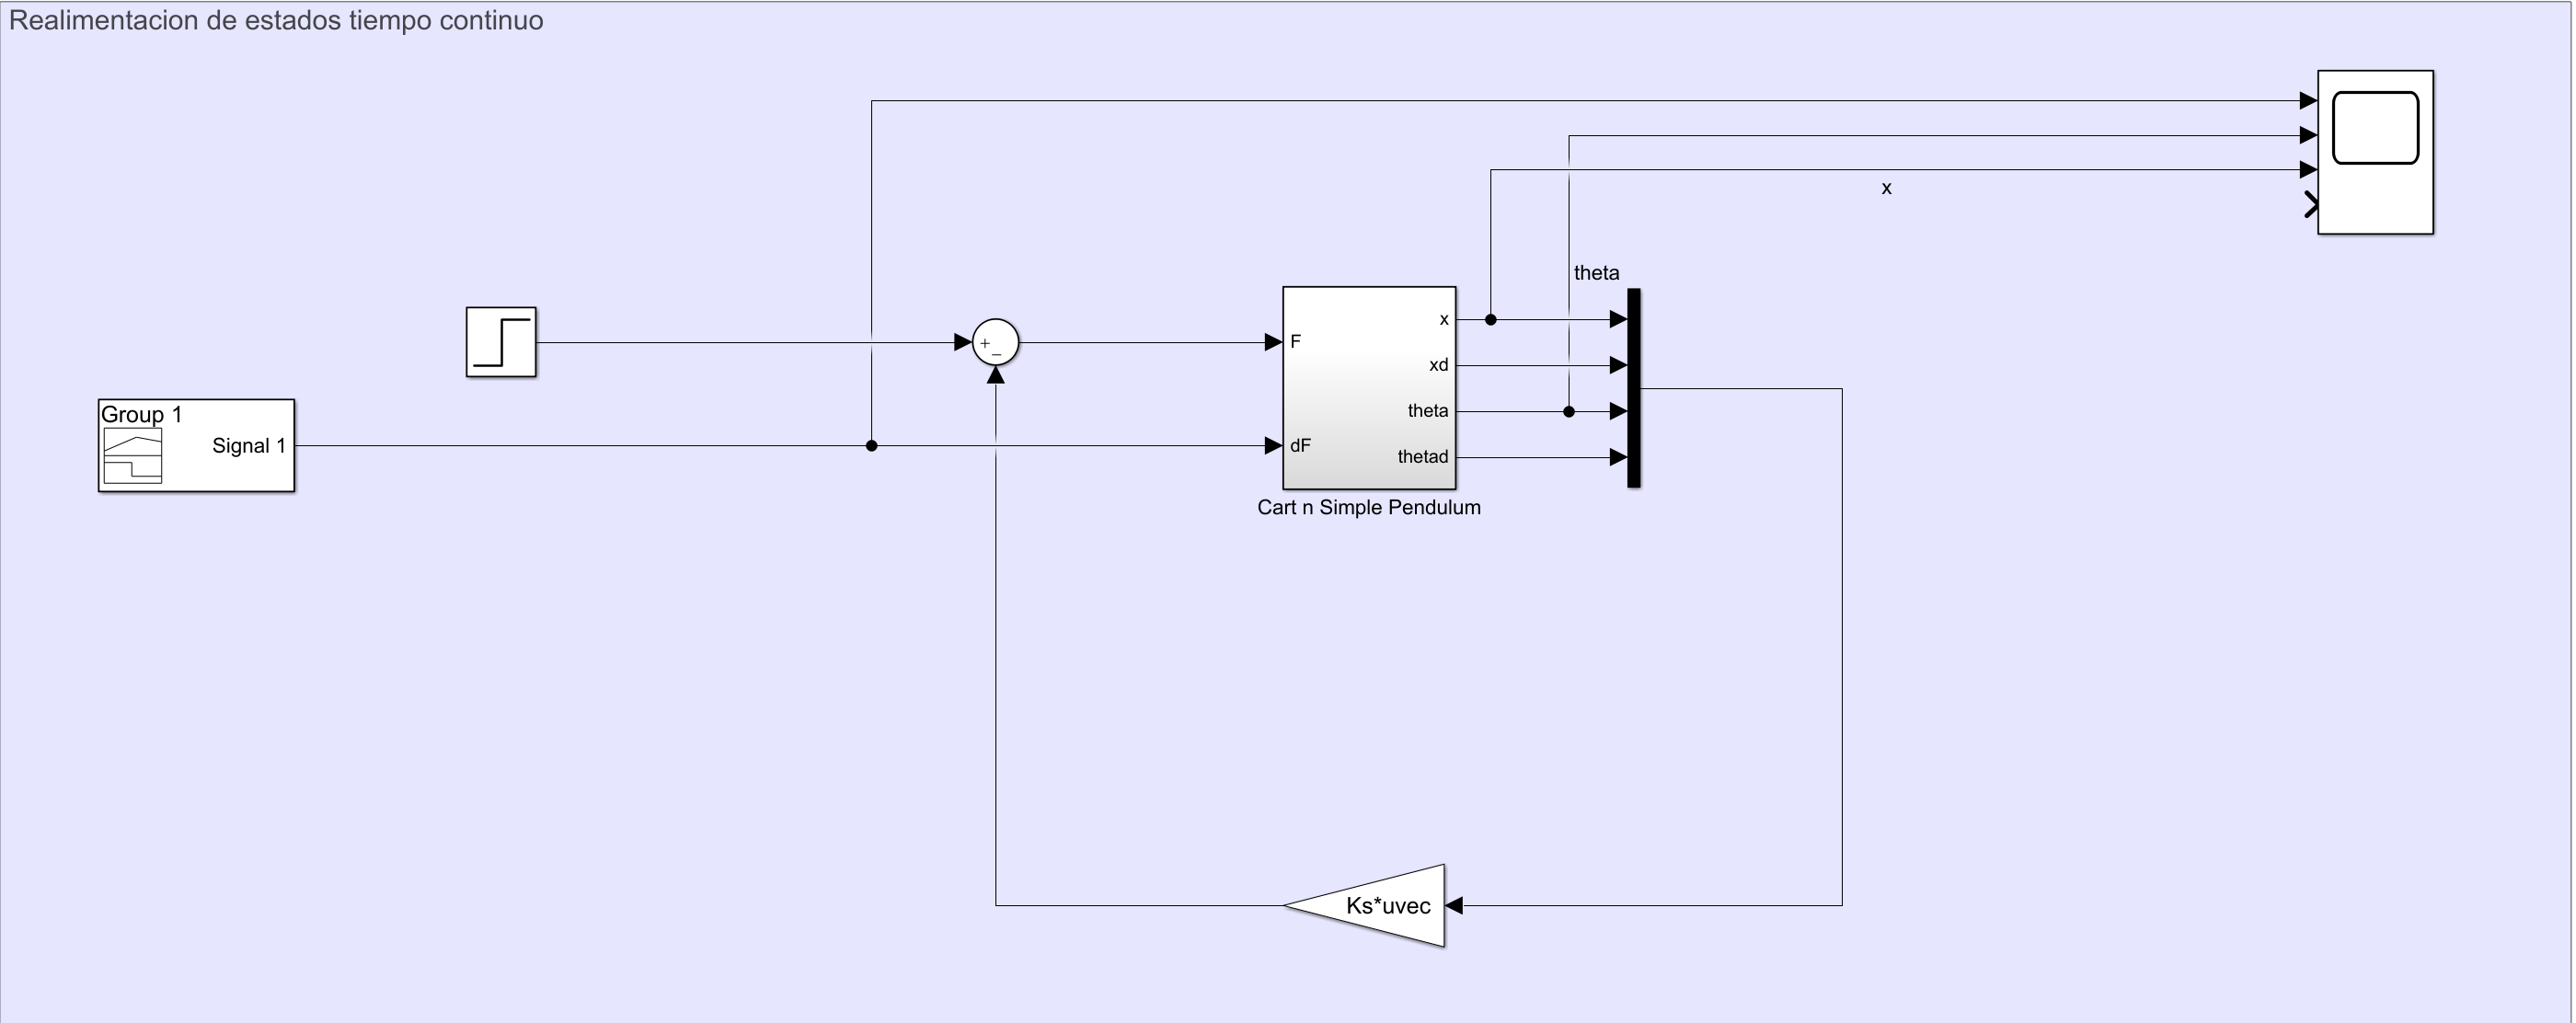
\includegraphics[width=0.8\linewidth]{ImagenesRealimentacióndeEstados/onlyFeed}
	\caption{Control por Realimentaci\'on de estados en tiempo continuo}	
	\label{fig:onlyFeed}
\end{figure}
Se muestra en la Figura \ref{fig:onlyFeedOut} tanto las salidas como las entradas del sistema. Puede observarse que tanto al aplicar el escal\'on inicial de fuerza como al aplicar un disturbio a los 4 segundos, el sistema es capaz de retornar a la posici\'on de equilibrio en un tiempo menor a 3 segundos para el caso de la mayor perturbaci\'on.
Se observa adem\'as, que el sistema tiene error permanente en la posici\'on del carrito, es por ello que se impementa a continuaci\'on la acci\'on integral
\begin{figure}[H]
	\centering
	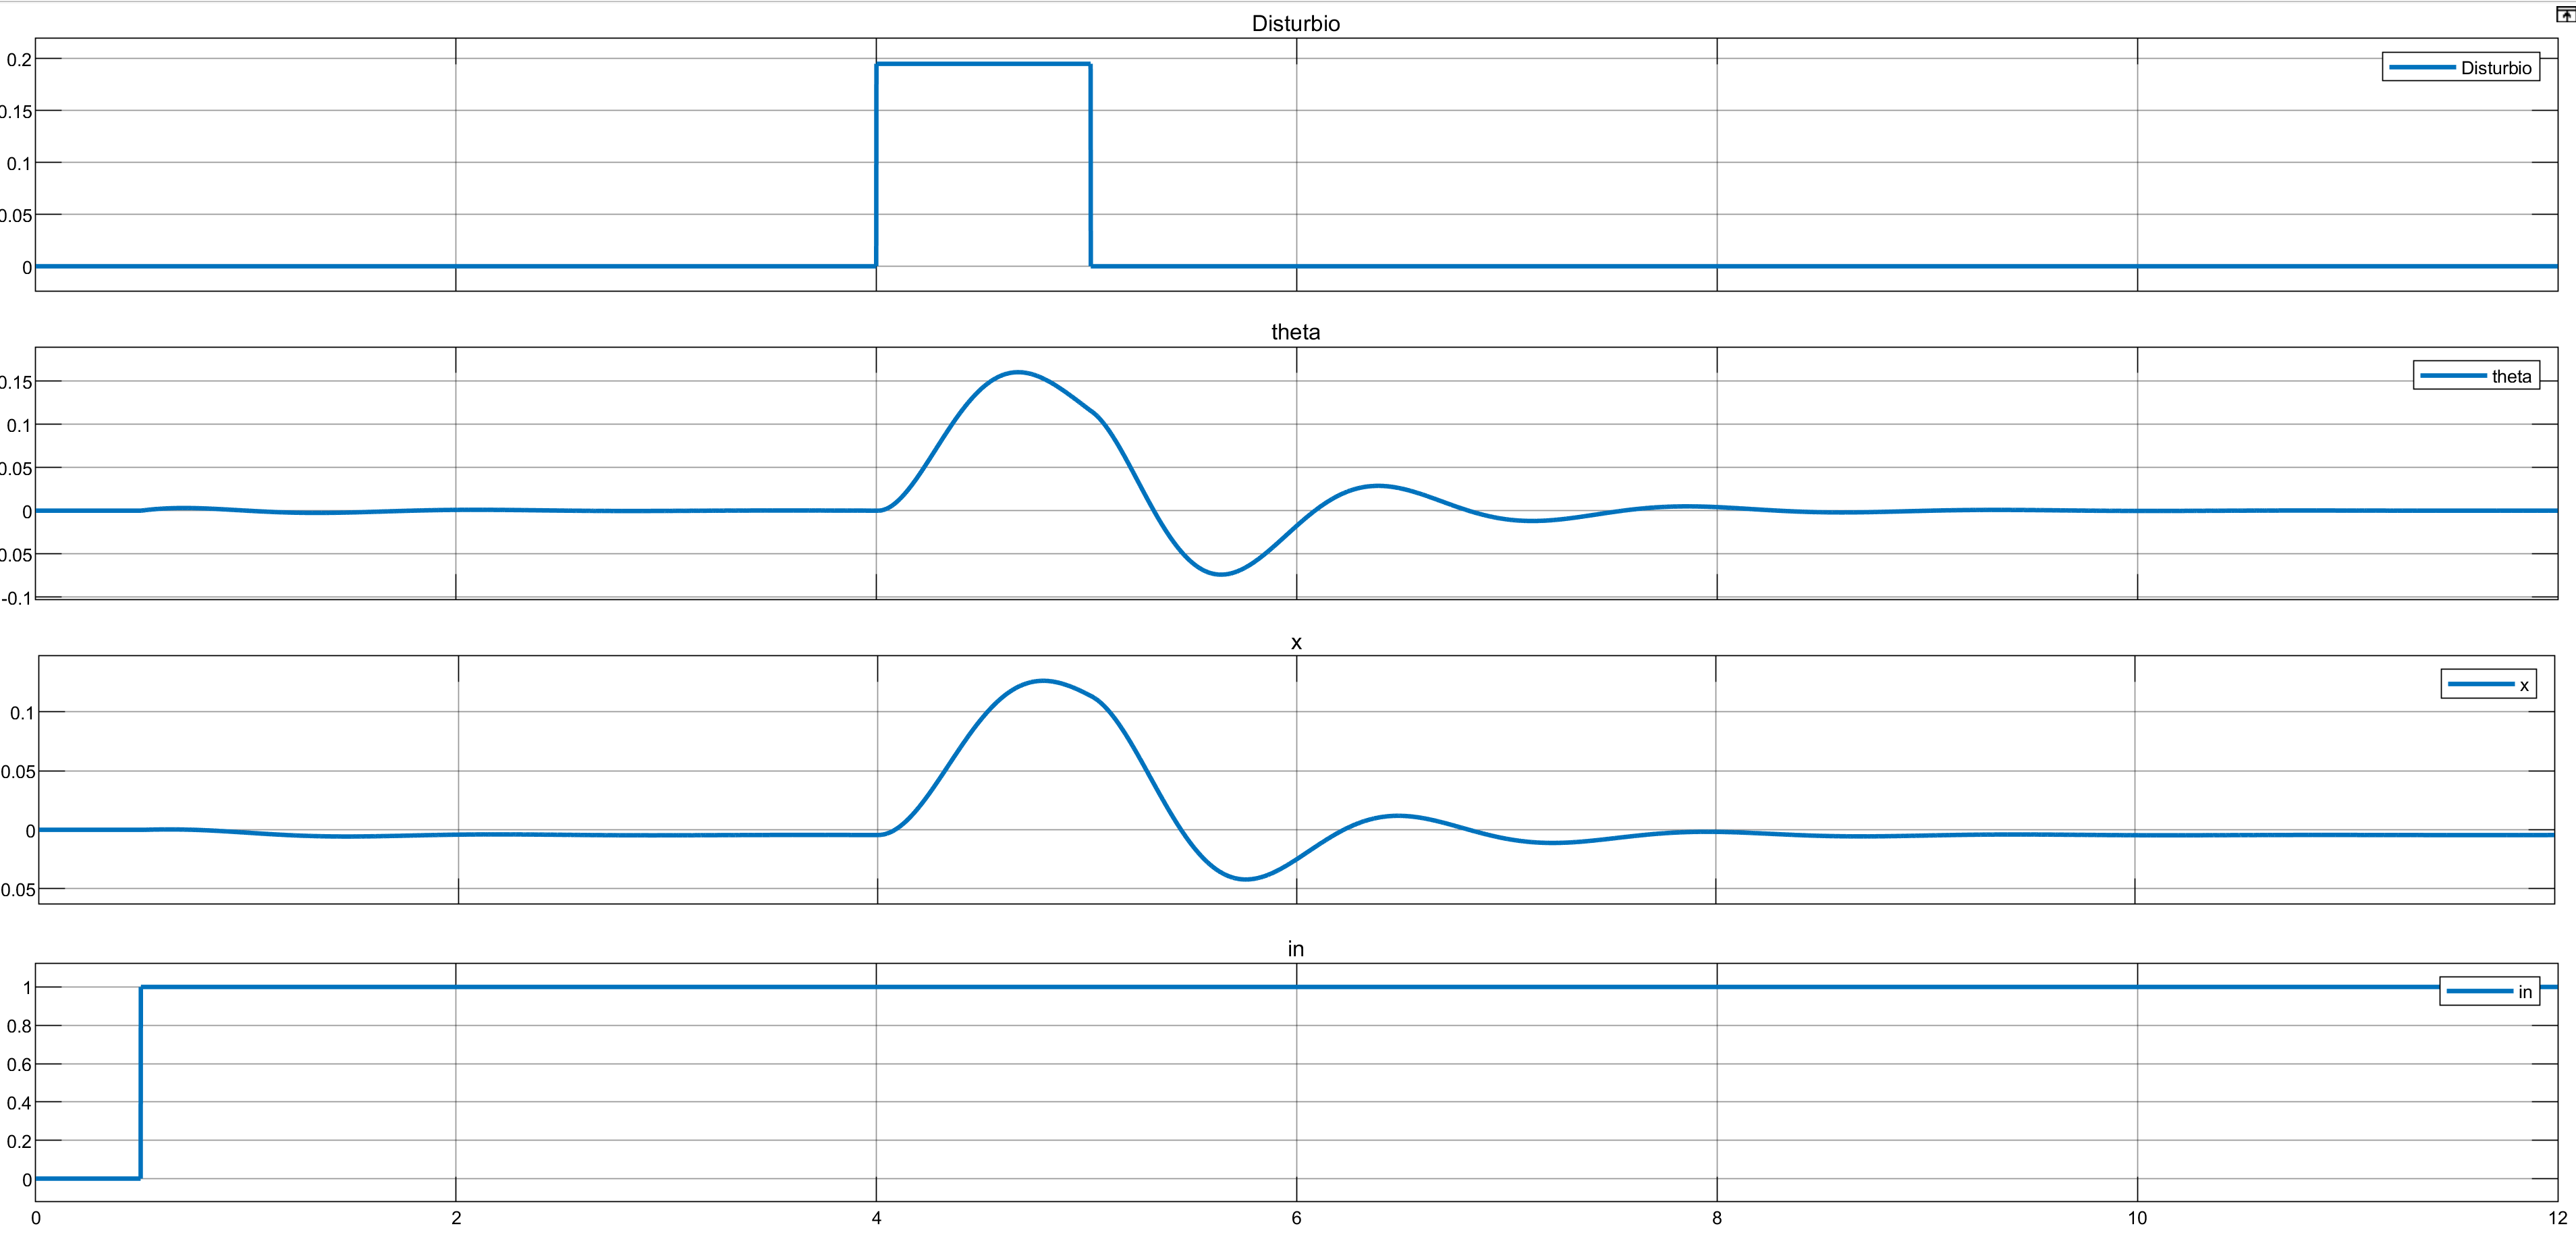
\includegraphics[width=0.8\linewidth]{ImagenesRealimentacióndeEstados/onlyFeedOut}
	\caption{Salidas y entradas del control por realimentaci\'on de estados en tiempo continuo}	
	\label{fig:onlyFeedOut}
\end{figure}

\subsection{Control integral en tiempo continuo}
Con el fin de elimininar el error permanente, se implementa el sistema con acci\'on integral como se ve en la Figura \ref{fig:integralFeed}. Cabe aclarar que se le agrega la posibilidad de cambiar la referencia del sistema, pudiendo asi seleccionar la posici\'on final del carrito respeto al origen.
\begin{figure}[H]
	\centering
	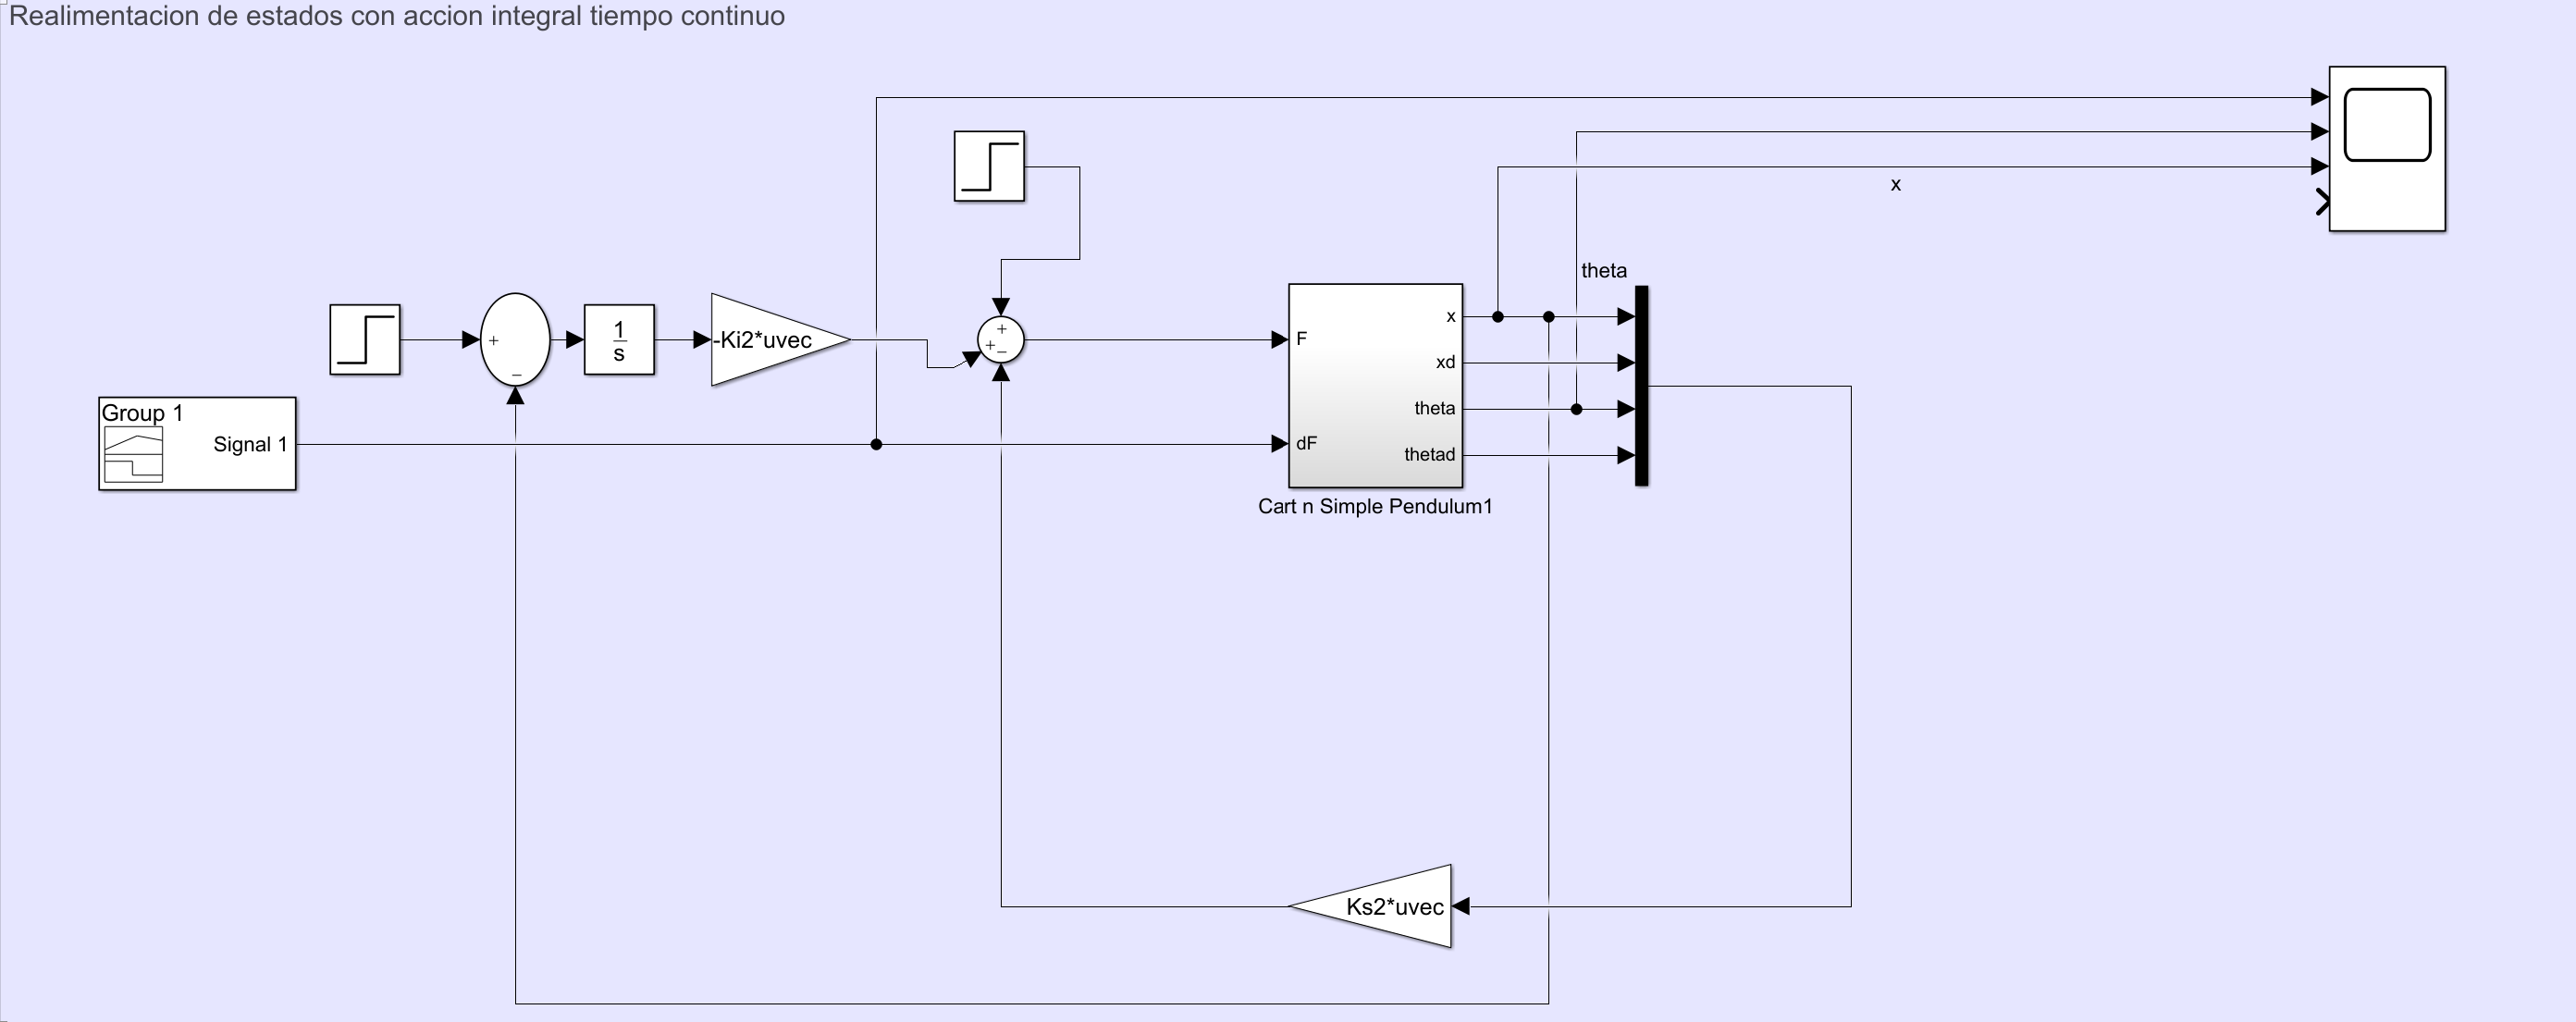
\includegraphics[width=0.8\linewidth]{ImagenesRealimentacióndeEstados/integralFeed}
	\caption{Control por Realimentaci\'on de estados con acci\'on integral en tiempo continuo}	
	\label{fig:integralFeed}
\end{figure}
Los polos del sistema se ubican teniendo cuidado de colocar 2 polos lentos relacionados con las variables de posicion y velocidad de carrito y 2 polos mas r\'apidos relacionados con el angulo y la velocidad angular del p\'endulo. En -3 y -15 respectivamente.\newline
Se muestran en la Figura \ref{fig:integralFeedOut}
\begin{figure}[H]
	\centering
	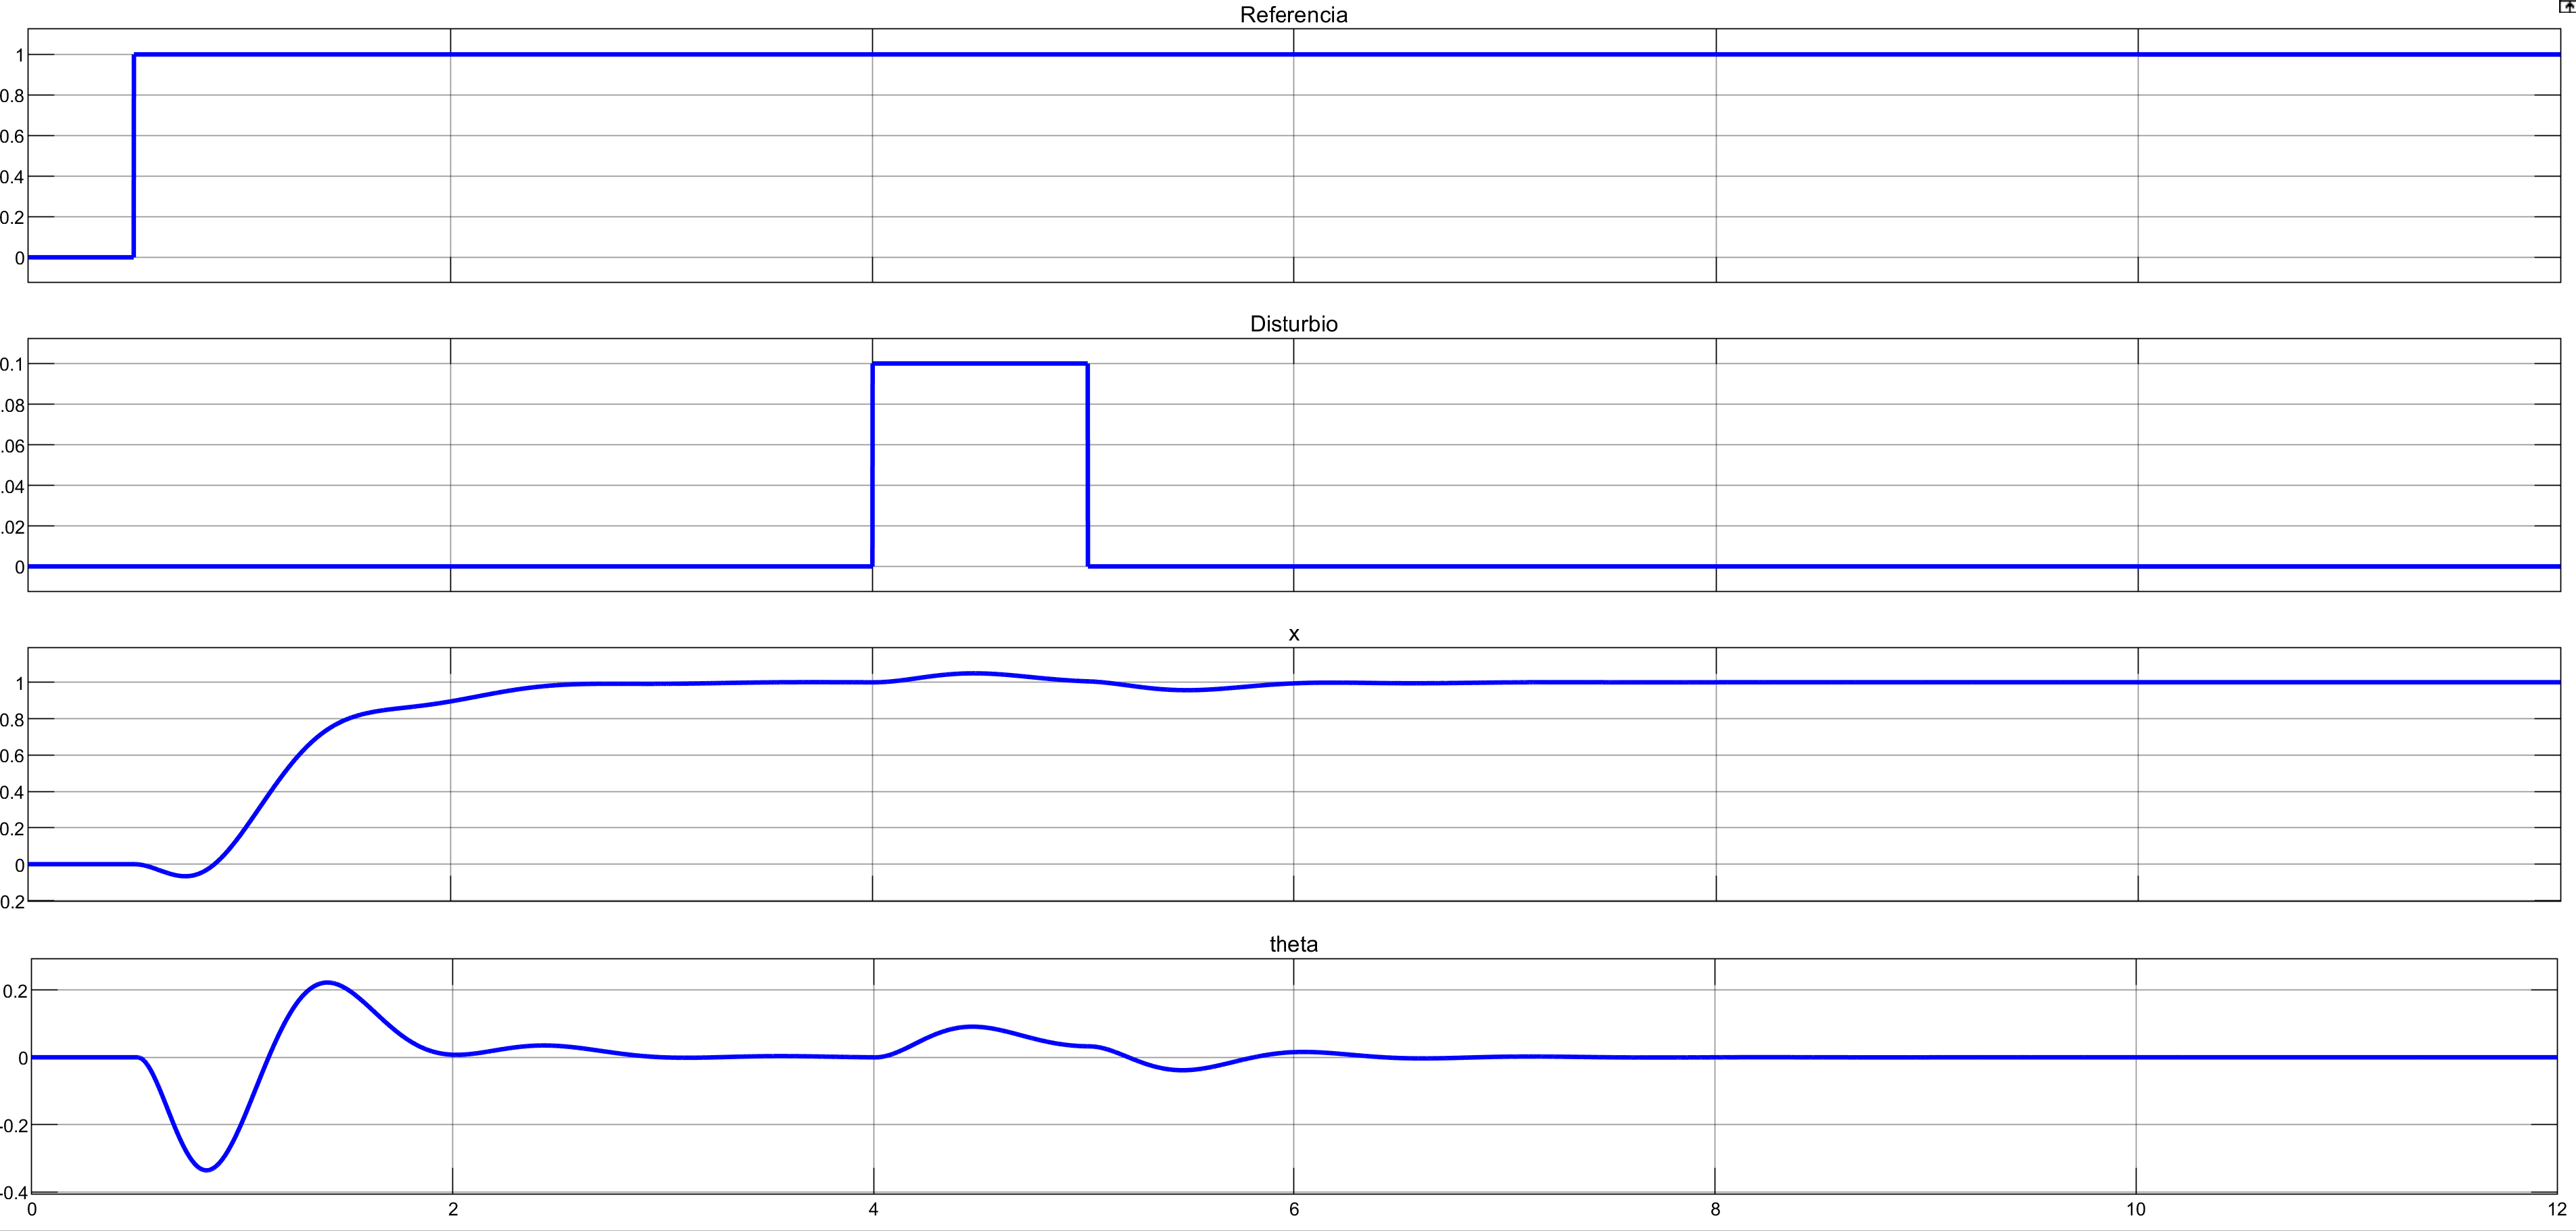
\includegraphics[width=0.8\linewidth]{ImagenesRealimentacióndeEstados/integralFeedOut}
	\caption{Entradas y salidas del Control por Realimentaci\'on de estados con acci\'on integral en tiempo continuo}	
	\label{fig:integralFeedOut}
\end{figure}
Se observa que el sistema se estabiliza rapidamente tanto al cambiar la referencia como ante un disturbio y en este caso se logra eliminar el error permanente.
\subsection{Control integral en tiempo discreto}
Por \'ultimo se implementa el sistema con acci\'on integral en tiempo discreto, utilizando un integrador discreto y los zero orer hold correspondientes, como e observa en la Figura \ref{fig:discreteIntegralFeed}
\begin{figure}[H]
	\centering
	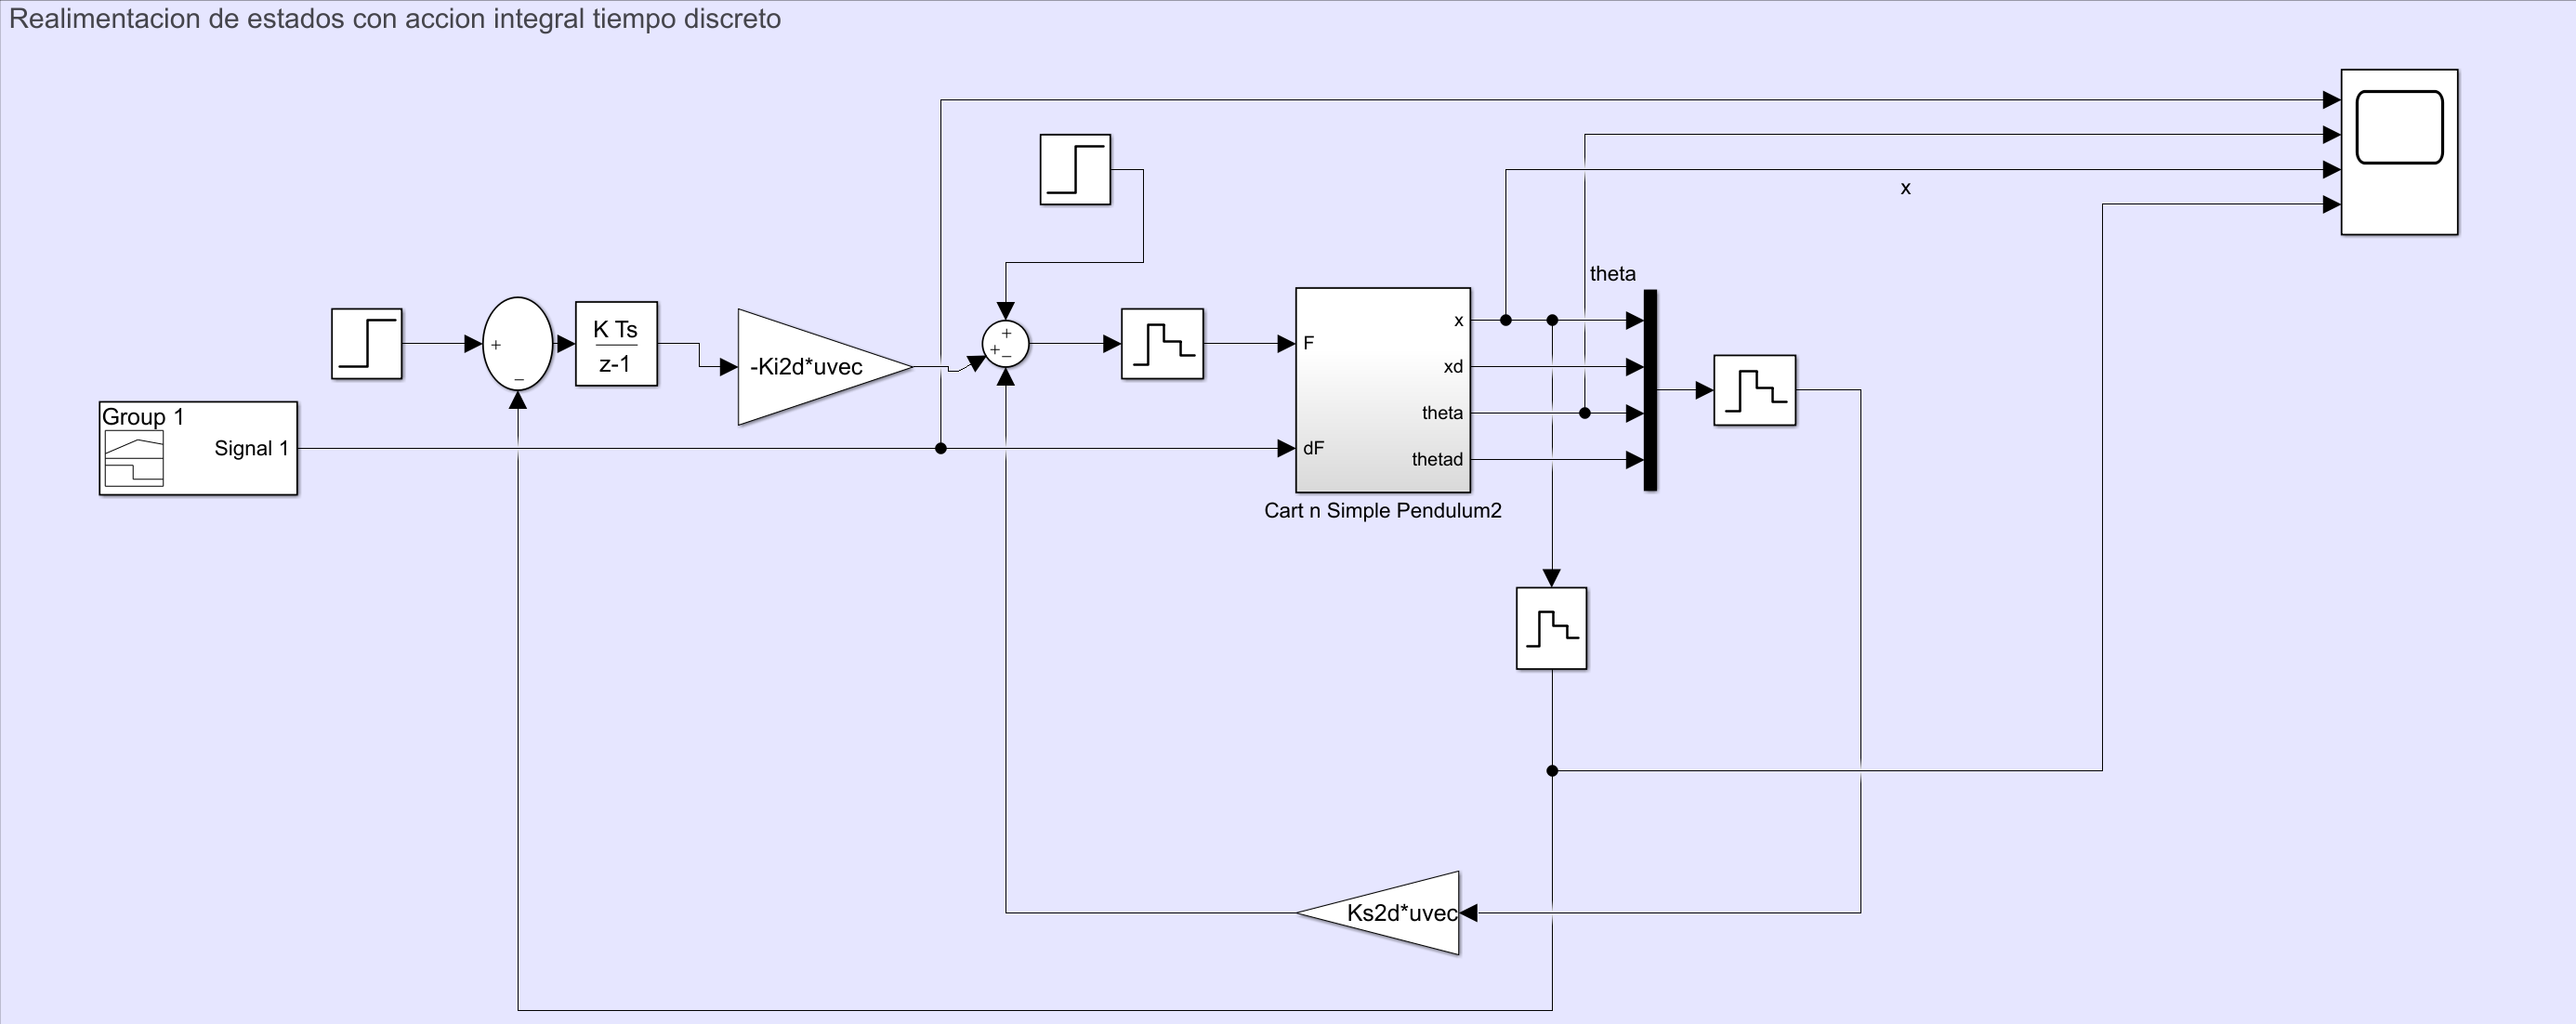
\includegraphics[width=0.8\linewidth]{ImagenesRealimentacióndeEstados/discreteIntegralFeed}
	\caption{Control por Realimentaci\'on de estados con acci\'on integral en tiempo discreto}	
	\label{fig:discreteIntegralFeed}
\end{figure}
Para ubicar los polos, se utiliza lqi(Lqr con acci\'on integral) dandole poca penalizaci\'o en la matriz Q a la posici\'on y a la velocidad del carrito y mucha al \'angulo en el que se encuentra. Adem\'as, se selecciona un tiempo de muestreo de 50ms. 
Conservando las entradas del caso anterior, se muestran las salidas del sistema continuo y su discretizaci\'on en la Figura \ref{fig:discreteIntegralFeedOut}
\begin{figure}[H]
	\centering
	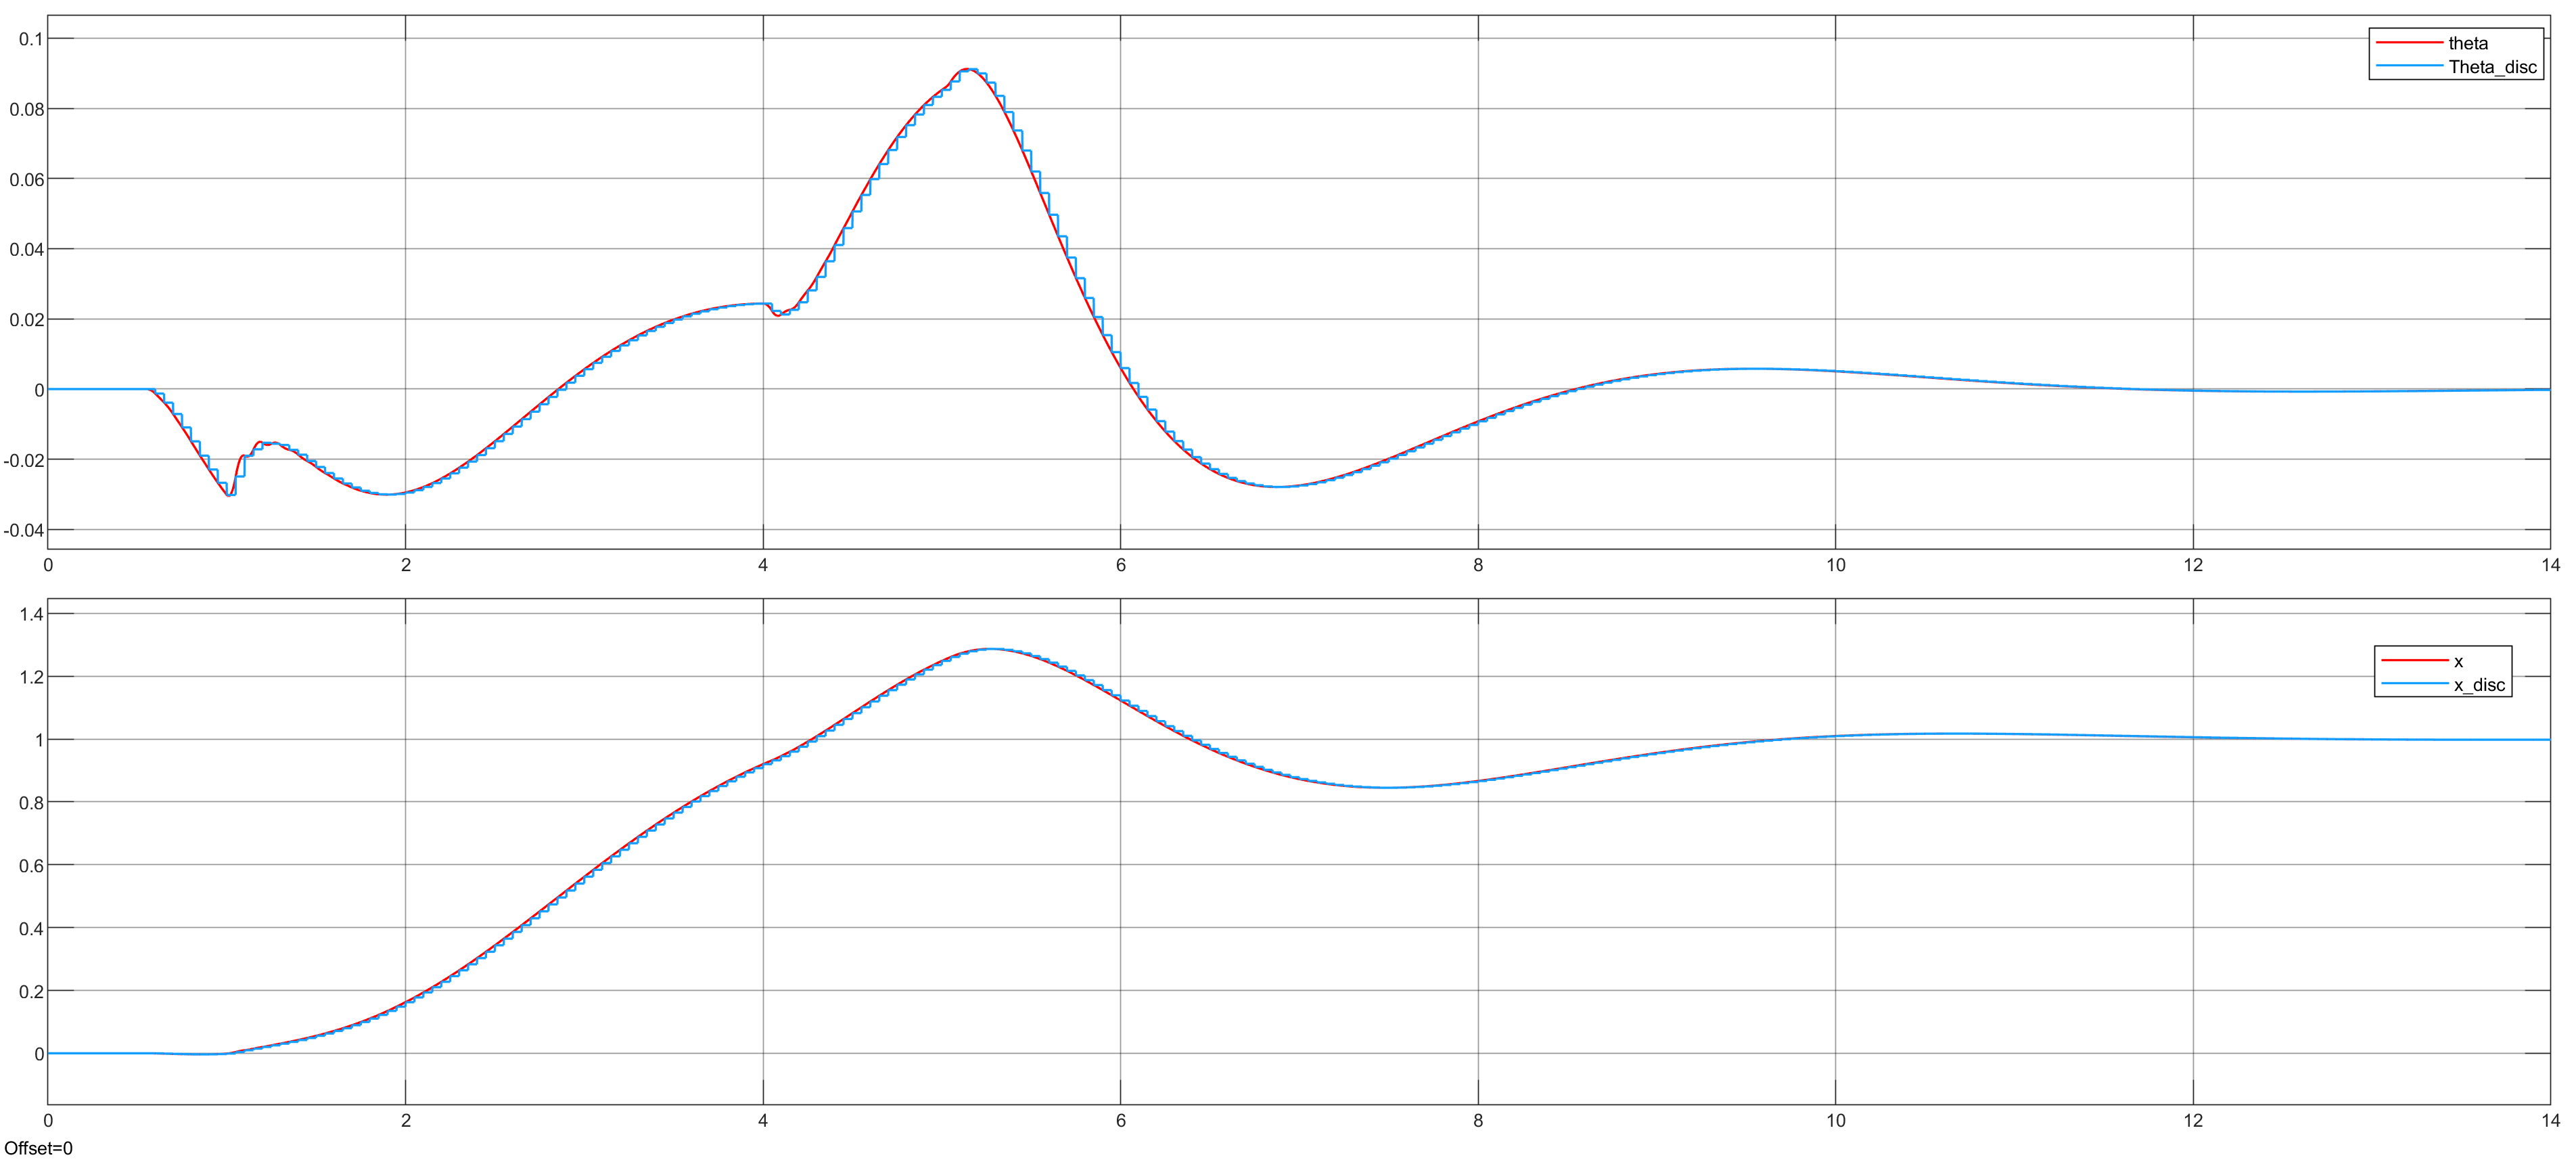
\includegraphics[width=0.8\linewidth]{ImagenesRealimentacióndeEstados/discreteIntegralFeedOut}
	\caption{Salidas del Control por Realimentaci\'on de estados con acci\'on integral en tiempo discreto}	
	\label{fig:discreteIntegralFeedOut}
\end{figure}
Se puede observar que en este caso el funcionamiento del sistema continua siendo correcto.
%\end{document}